\documentclass[11pt]{article}
\usepackage[paper=a4paper, left=1cm, right=1cm, bottom=1.5cm, top=1.5cm]{geometry}

\usepackage{sectsty}
\usepackage{graphicx}
\usepackage{listings}
\usepackage{amsmath}
\usepackage{xcolor}
\begin{document}
\tableofcontents

\section{Previa-practica}
Especificar es describir un tipo de datos a traves de sus operaciones, su comportamiento,
lo que podemos observar.
Si yo me pregunto que es un diccionario, podria responder que es un tipo de datos
que mapea elementos de tipo  $\alpha$ a tipo de elementos $\beta$.

Vamos a querer una estrucutra y algoritmos que responden a la especificacion.
La interfaz de un modulo es una capa intermedia entre las estructuras y algoritmos
que implementan el tipo de datos y el usuario de los mismos.

La funcion de abstraccion recibe una instancia de una estructura y devuelve una
instancia de un TAD.
Para esto tiene que valer el invariante de representacion, es decir
la estructura tiene que estar bien formada.
Nosotros vamos a definir la serie de restricciones que tiene que tener la estructura
para que sea valida o no.

\begin{figure}[h!]
    \centering
    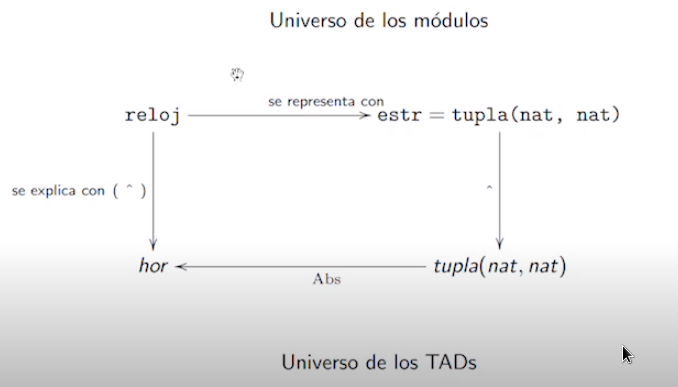
\includegraphics[width=0.7\textwidth]{absres.png}
\end{figure}

El invariante es la pre y poscondicion de cada una de las operaciones que define
nuestra interfaz.
Las operaciones estas van a asumir que cualquier estructura que venga va a venir
ya bien formada, valida.
Y asegura que cualquier estrucutra que salga lo va a ser bien formado.


\section{Dise\~no}
Diseñar: Preguntarnos el como.

Hay muchos comos posibles. Ver como elegir uno.
Consideraremos aspectos no funcionales como la eficiencia en tiempo y espacio.
Como tambiene l encapsulamiento y ocultamiento de informacion.

En general el como nos va a dar diferentes complejidades para cada funcion.
Dependiendo del uso que vamos a darle es el que vamos a usar.

Por ejemplo, si quiero diseñar al TAD conjutno, podemos pensar en dos implementaciones.
Un arreglo redimensionable ordenada. Cada vez que se me llena pido mas memoria.
Mantengo un puntero al ultimo elemento, y cada vez que agrego(sin repetidos)
uno miro a donde tiene que ir, muevo e inserto (O(n)).
Como esta ordenado, la busqueda (usando busqueda binaria) es O(logn).
Por el otro lado puedo hacer una secuencia (no esta ordenado).
Entonces la insercion es o(1) (simplemente lo meto), encambio la busqueda,
se hace en forma O(n) ya que al no estar ordenada tengo que recorrer todo.

En esta etapa, nos centramos en el como y no el que.
Para eso hacemos cambio de paradigma, de funcional de la especificacion al imperativo
del programa.
Necesitamos proveer una representacion para los valores, definir las funciones del
tipo y demostrar que es correcto.

Lo que usaremos es el dise\~no jerarquico.
Es decir vamos a pasar de la especificacion a la implemetacion de forma ordeanada
o jerarquica.
Por ejemplo podriamos pasaremos de un conjunto de naturales a representarlos
con una secuencia de naturales y luego con punteros.

Dependiendo del contexto podremos elegir que solucion vamos a tomar.
Para poder hacer esto, vamos a usar una metodologia de dise\~no.
El primer paso es la eleccion del tipo a dise\~nar.
En general usaremos el concepto de \textit{top down}, es decir el TAD mas abarcativo.
Luego vincularemos la presentacion con su abtraccion.
Y por ultimo iteraremos sobre los tipos restantes.

Hay dos claros aspectos:
\begin{itemize}
    \item Aspectos de la interfaz: desceriben todo elemento relacionado con los aspectos
        de uso de dicho tipo.
        Todo lo visible desde afuera.
    \item Pautas de implementacion: todo aspecto que refiera a cuestiones vinculadas
        a los medios a traves de los cuales el tipo garantiza esos aspectos de uso.
        Como se implementa.
\end{itemize}

Con el aspecto interfaz de un modulo de dise\~no implica explicarle a un usuario
los aspcetos relativos a los servicios que ese modulo que estamos dise\~nando exporta.

\begin{itemize}
    \item Servicios exportados: describe para cada operacion su complejidad, aspectos
        de aliasing, efectos colaterales sobre los argumentos, etc.
    \item Interfaz: define en el paradigma imperativo las operaciones exportadas
        junto con su precondicion y postcondicion.
        Esto establecera la relacion entre la implementacion de las operaciones
        y su especificacion.
\end{itemize}

Cosas que nos pueden pasar durante este proceso, es la necesidad de cambiar la aridad
de una funcion.
O ver decidamos que algunas funciones se mergeen o que se dividan.

\paragraph{Transparencia referencial} es cuando su resultado solo de sus parametros
explicidos.
Es decir cuando no llamo a otra funcion o lo que fuera para poder dar el resultado.
En el paradigma funcional, todas las funciones son transparentes referenciales,
no asi en el paradigma imperativo.
\paragraph{aliasing}: significa la posibilidad de tener mas de un nombre para
la misma cosa.
Dos punteros o referencias hacia el mismo objeto.
Ej: si hago una funcion \textit{podar} para un arbol binario, la cual dado un arbol
me devuelve el sub arbol izquierdo y derecho.
Si al hacerlo me devuelve una referencia de ambos, esto es aliasing (no esta mal,
si no que hay que aclararselo al usuario, como tambien si se lo devuelvo por copia).
Ya que si no el usuario si piensa que es por copia, al luego modificarlo, estaria
modificando todo (el arbon original).
Si fuera al reves que el usuario cree que es por refernecia y en realidad es por copia,
posiblemente el usuario se cree una copia previa para evitar futuras modificaciones
al mismo generando una doble copia sin sentido.

En general, en la interfaz, uno dice para cada funcion si produce o no aliasing o efectos colaterales
sobre los argumentos, la complejidad y lo que significa ese parametro de complejidad n.
Si por ejemplo tengo una funcion de conjunto que es agregar un elemento, al recibir
como parametro al propio conjunto y lo devuelve modificado (se le agrego un nuevo elemento)
esto seria con efectos colaterales sobre los argumentos.

\paragraph{Ocultar informacion}
Nociones:
\begin{itemize}
    \item Abraccion: el proceso de identificar los aspectos importantes de un
        fenomeno ignorando los detalles.
    \item Ocultamiento de la informacion: cada modulo tiene que revelar lo menos posibles
        su funcionamiento interno.
        De esa forma disminuye la interferencia con otras partes del sistema.
    \item Encapsulamiento: el usuario tiene la visibilidad total sobre los procedimientos
        sobre un cierto objeto pero sin visibilidad de sus datos.
        Solo puede acceder a sus datos o modificarlos a traves de los procedimientos.
\end{itemize}

Las ventajas de esto son, que ayuda el poder mejorar cambiando una implementacion
sin afectar su uso.
Ayuda a modularizar y a facilitar la comprension y reuso.
Generando tambien que el sistema sea mas resistente a los cambios.

\subsection{Relacion imperativo y logico}

Vamos a resolver este problema introduciendo una funcion que para cada volor imperativo
nos retornara un termino logico al cual representa, de forma que este pueda participar
de los predicados logicos que definen el comportamiento formal de las operaciones.
Esta funcion es el sombrero.
Nos permitira poder usar el operador de igualidad observacional entre algo imperativo
(al que le aplicaremos el sombrerito) con algo funcional (los TADs).

\subsection{Representacion}
El camino a seguir:
\begin{itemize}
    \item Estructura: describe la estructura interna sobre la cual las operaciones aplican.
    \item Relacion entre representacion y la abstraccion: expone toda restriccion sobre
        la estructura de representacion a fin d e que efectivamente pueda ser consiederada
        una implementacion de un valor del tipo al que implementa y por otro lado
        vincula los valores con su contraparte abstracta (con algun termino de la especificacion
        a quien este represente).
    \item Algoritmos: la programacion en pseudo-codigo de las operaciones, tanto
        las exportadas como las auxiliares e incluyendo para todos ellos el calculo
        detallado que justifica su complejidad.
    \item Servicios usados: declara toda demanda de complejidad, aliasing o efecto
        colateral que los servicios usados de otros tipos en la programacion de
        los algoritmos deban satisfacer.
\end{itemize}

\paragraph{Estructura de representacion} describew los valores sobre los cuales
se representara el genero que se esta implementando.

Ej: implementar conjunto semi rapido. Implementar conjunto de naturales donde
del numero 1 al 100 deban manejarse en o(1) y el resto en O(n). Ademas quiero
concer la cardinalidad del conjunto de forma rapida.
Lo que tiene que quedar claro es que esto siegue siendo el TAD conjunto.

Porpuesta: un arreglo de 100 posiciones booleanas, una secuncia y un nat para la
cardinalidad.
Esto lo escribimos de la siguiente manera:

Conj\_semi\_rapido\_nat  \textbf{se representa con} (\texttt{src})
tupla$<$rapido:arreglo \[1..100\] de bool x resto: secu(nat)xcant: nat$>$.

\paragraph{Invariante de representacion}.
Preguntas, podemos representar cualquier conjunto con esta representacion? Si.
Cualquier cosa de esta pinta, representa un conjunto? No.

Veamos el no con un contraejemplo.
$<\left[0..0\right], <>, 8245>$
no es un conjunto semi rapido de naturales.
La cardinalidad es mayor a cero y el conjunto no tiene ningun elemento.
Otro seria
$<\left[0..0\right], <37, 107, 28>, 3>$.
En este caso la cardinaldida se cumple, pero tenemos en resto elementos que deberian ir en rapido.

Estas cosas son postcondiciones que tienen que garantizar cualquier algoritmo
de nuestra estrucutra. Lo mismo para la precondicion.

El Invariante de representacion, es una funcion booleana con dominio en el genero de
representacion que da true cuando recibe una instancia valida.
El dominio es la version abstracta del genero de representacion, es decir
aplicando el sombrerito.

Si representamos un tipo abstracto $T_1$ sobre uno mas concreto $T_2$, se escribe asi:

Rep:$\hat{T_2} \rightarrow bool$

($\forall:\hat(T_2)$)Rep(t) $\equiv$ condiciones que garanticen que t representa
una instancia valida de $T_1$.

En nuestro ejemplo seria:
\begin{figure}[h!]
    \centering
    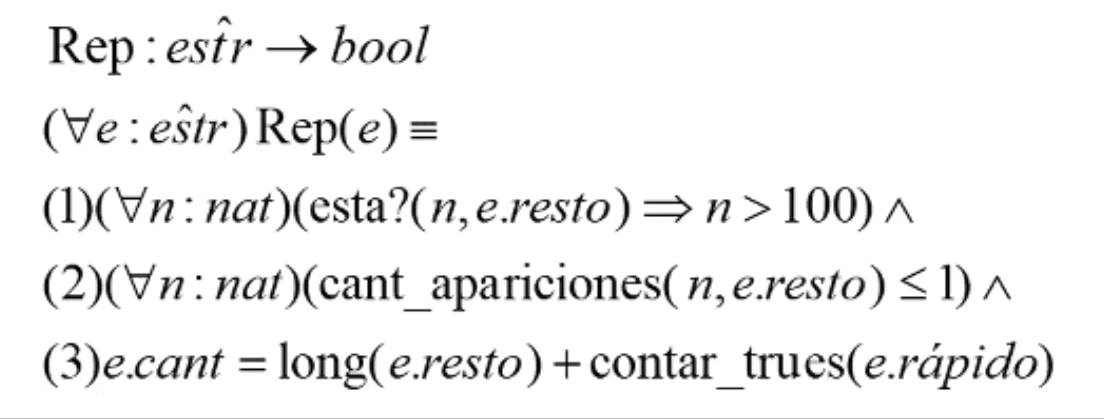
\includegraphics[width=0.7\textwidth]{rep.png}
\end{figure}

\subsection{Funcion de abstraccion}
Vincula una estructura con algun valor abstracto al que representa.

Abs:$\hat{T_2}e \rightarrow \hat{T_1}(Rep(e))$.

Toma una instancia abstracta de la  estructura de representacion y devuelve una
instancia abstracta pero del genero representado.

\begin{figure}[h!]
    \centering
    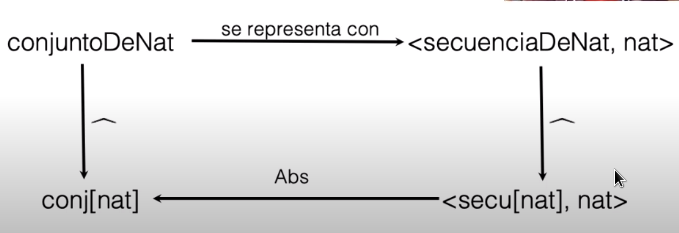
\includegraphics[width=0.7\textwidth]{abs.png}
\end{figure}

\begin{figure}[h!]
    \centering
    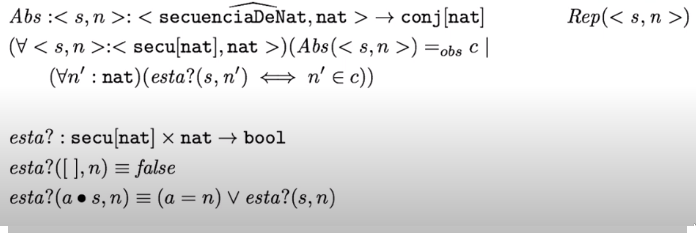
\includegraphics[width=0.7\textwidth]{absEj.png}
\end{figure}

\begin{figure}[h!]
    \centering
    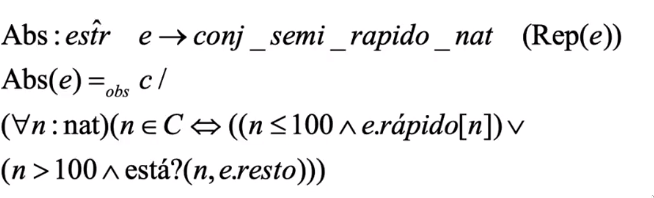
\includegraphics[width=0.7\textwidth]{abs2.png}
\end{figure}

Propiedades:
\begin{itemize}
    \item Una vez restringida a (Rep(e)), debe ser total.
    \item No tiene por que ser inyectiva: Dos estructuras diferentes
        pueden representar al mismo termino de un TAD.
    \item Debe ser suryectiva (subyectiva) sobre las clases de equivalencia determinadas
        por la igualdad observacional, restringidas a lo especificado por el contexto
        de uso. Todos los elementos son mapeados a algo.
    \item No tiene por que ser subyectiva sobre todos los terminos del genero
        representado.
\end{itemize}


\begin{figure}[h!]
    \centering
    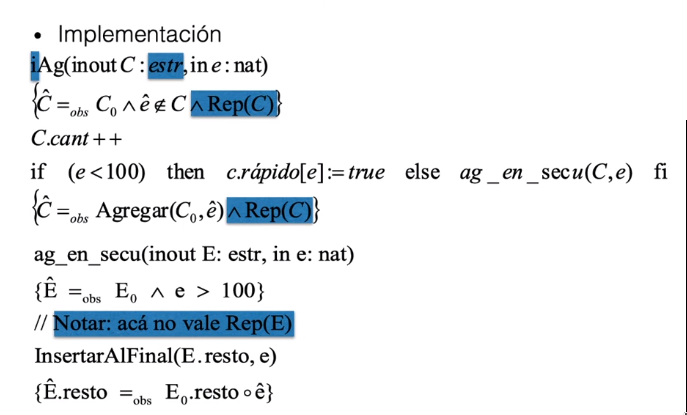
\includegraphics[width=0.7\textwidth]{algo.png}
\end{figure}


\section{Sorting}
Ordenar un arreglo de $\alpha$, el cual es un tipo
que esta definida la relacion $<_{\alpha}$.

Un algoritmo es \textbf{estable}, si mantiene el orden anterior de elementos
con igual clave.
Es decir si tengo un arreglo de tuplas, y ordeno por el primer  elemento.
Un algortimo estable va a precerbar el orden original del segundo elemento, mientras
que uno inestable no me lo garantiza.
Ej:

\begin{centering}
Original  \hspace{0.8cm} Estable \hspace{0.8cm} inestable

\textcolor{red}{(9,7)}  \hspace{1cm} (4,1) \hspace{1cm} (4,1)

(5,3) \hspace{1cm} (5,3)\hspace{1cm} (5,3)

(4,1) \hspace{1cm} (5,2)\hspace{1cm} (5,2)

(5,2) \hspace{1cm} \textcolor{red}{(9,7)} \hspace{1cm} \textcolor{red}{(9,2)}

\textcolor{red}{(9,2)} \hspace{1cm} \textcolor{red}{(9,2)} \hspace{1cm} \textcolor{red}{(9,7)}

Esto tiene mucha utilidad si primero ordeno por los primeros elementos y luego
por los segundos.
Ejemplo tupla apellido nombre. Primero ordeno por apellido y luego por
nombre.
Si el algoritmo fuera inestable, al ordenar luego por nombre, me
romperia el orden que ya hice de los apellidos.
\end{centering}

\begin{figure}[h!]
    \centering
    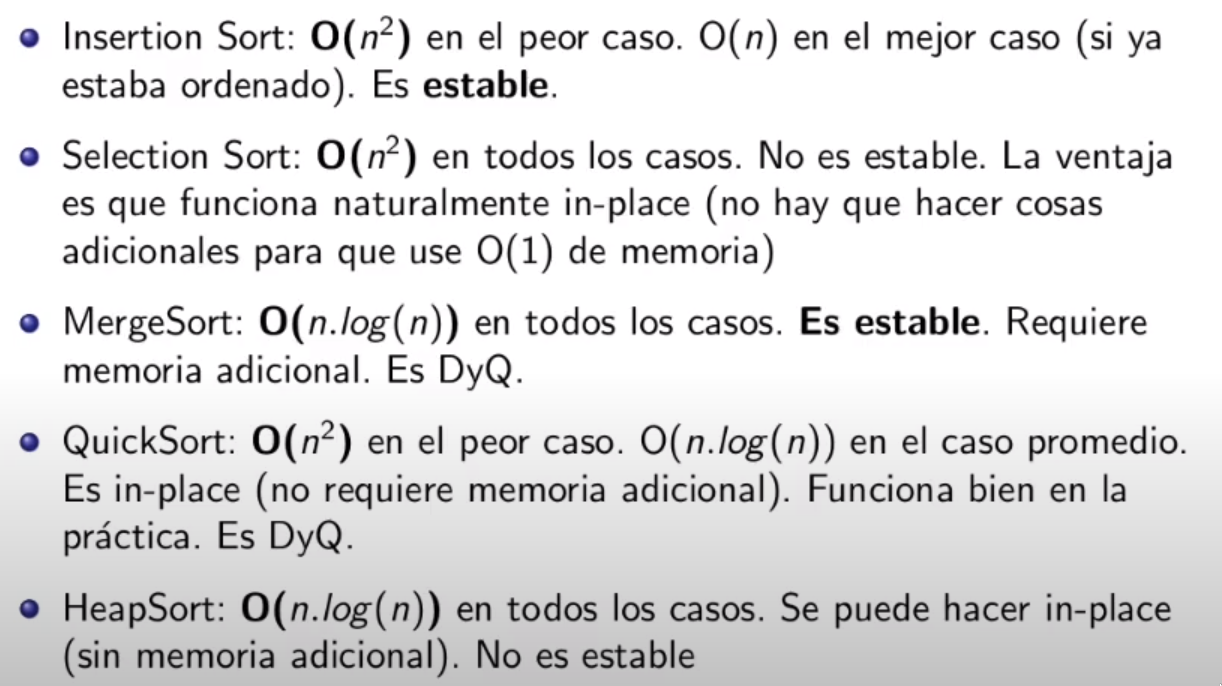
\includegraphics[width=0.7\textwidth]{sortResumen.png}
    \caption{Resumen de los diferentes algoritmos.}
    \label{fig:res}
\end{figure}


\subsection{Selection sort}
Ordenamiento por seleccion.
Basicamente arranco a mirar todo el arreglo buscando el minimo.
Al encontrarlo lo swapeo al principio del arreglo y arranco
nuevamente la busqueda pero obviando el primer elemento.
Repito hasta el anteultimo.
Al swapear estoy llevando el primer elemento del recorrido, a la
posicion de donde esta el minimo.

\paragraph{Invariante:} En la iteracion i-esima vamos a tener que a la izquierda
de la posicion i del arreglo van a estar todos los elementos
mas chicos y ordenados y para la derecha van a estar simplemente
los elemenos mas grandes.
Ademas todo el arreglo sin importar la iteracion es una permutacion
del arreglo original, ya que no estoy agregando ni sacando nada.

\begin{figure}[h!]
    \centering
    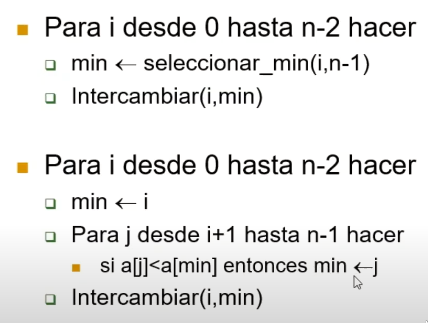
\includegraphics[width=0.7\textwidth]{selection.png}
    \caption{Pseudo-codigo del algoritmo Selection Sort.}
    \label{fig:selection}
\end{figure}

\paragraph{Complejidades:}
Basciamente es ir buscando un minimo en un arreglo cada vez mas chico.
Para la i-esima iteracion, tendremos un costo de O(n-i-1).
\begin{align*}
    \text{Costo} = \sum_{i=0}^{n-2}(n-i-1)=\sum_{i=1}^{n-1}i=\frac{n(n-1)}{2}\sim O(n^2)
\end{align*}

Por como esta es un algoritmo inestable.
\subsection{Insertion sort}
Empieza desde el segundo elemento, y se fija si es menor que el primero,
si lo es guarda en una variable dicho valor, y reemplaza el valor del primer
elemento en la segunda posicion y luego copia el valor guardado en la
primer posicion.
Pasa al tercer elemento, y compara primero con el segundo (si es menor
repite proceso) y luego compara con el primero y repite proceso.
Asi sucesivamente con todos.

\paragraph{Invariante:}
Los elementos entre la posicion 0 y la posicion i siguen siendo
los mismos pero permitiendo que tengan otro orden.
En esa parte estan todos ordenados.
Nuevamente el arreglo es una permutacion del original.

\begin{figure}[h!]
    \centering
    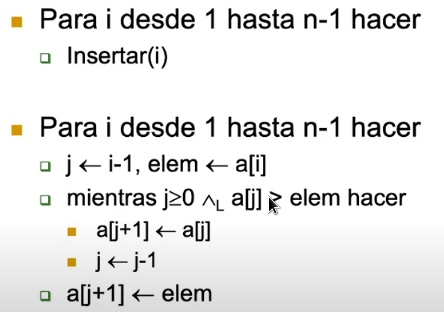
\includegraphics[width=0.7\textwidth]{insertion.png}
    \caption{Pseudo-codigo del algoritmo Inserion sort.}
    \label{fig:insertion}
\end{figure}


\paragraph{Complejidades:}
Dado un arreglo de n elementos, el ciclo pirncipal se ejecutara n-1 veces.
En el i-esima iteracion hay que ubicar al elemento junto a otros  i-1
elementos y por lo tanto necesitamos i-1 comparaciones.
\begin{align*}
    \text{Costp}=\sum_{i=1}^{n-1}i-1=\frac{(n-1)(n-2)}{2}\sim O(n^2)
\end{align*}

Si el arreglo esta parcialmente ordenada, las cosas mejoran.
Ya que no tiene que siempre mover hasta el primer elemento
cada iteracion.

Dicho algoritmo es estable.

\subsection{HeapSort}
Es una modificacion del Selection sort pero usando como estructura
de datos a un heap (cola de prioridad) para poder hacer la busqueda de minimo
en tiempo logaritmico.

La primer forma basica de este algoritmo (despues se complejiza)
es insetar cada elemento del arreglo en un heap ($\sum_i log(i)\sim nlog(n)$) y luego vamos
sacando (que devuelve siempre el minimo). Lo malo es requiere
de dos arreglos, uno el original y el otro en donde vamos armando
el heap.

La forma de mejorar esta version es utilizando el algoritmo de Floyd
el cual transforma un array en un heap en O(n).
Esto ademas hace que utilice un unico arreglo.

\begin{figure}[h!]
    \centering
    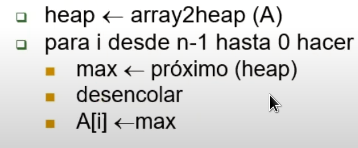
\includegraphics[width=0.7\textwidth]{heapsort.png}
    \caption{Pseudo-codigo del algoritmo de HeapSort}
    \label{fig:heapsort}
\end{figure}

La idea es que me armo un heap al reves de lo que quiero,
es decir si quiero de menor a mayor me armo un maxHeap.
Luego voy desencolando el primer elemento (el maximo) y lo
agrego al final del arreglo que es la memoria que se me libero.
Al hacer esto n veces me queda armado el arreglo de minimo a maximo.

\paragraph{Algoritmo de Floyd:}
Agarra el arreglo y lo piensa como una estructura de arbol heap.
Agarra al ultimo nodo con hijos y lo transforma (si es que hace falta) en heap (max o min).
Esto lo hace con la operacion bajar, es decir swapea el nodo con el hijo que
es el mayor o menor.
Luego mira a su vecino y vuelve a transformarlo en heap.
Asi hasta terminar el ultimo nivel.
Luego sube un nivel y aplica (si es necesario) la operacion bajar
hasta que quede un heap esa porcion del arbol y pasa a su vecino.
Cabe aclarar que ahora puede darse el caso de requerir aplicar
bajar dos veces.
Esto lo hago hasta llegar a la raiz.
Entonces en el peor caso voy a aplicar la operacion bajar la maxima
cantidad posible en cada iteracion.
Esto es (\# nodos en el penultimo nivel)1+ (\# nodos en el antepenultimo nivel)2+
...+(\#nodos en el nivel 2)(k-2)+(\#nodos en el nivel 1)(k-1)=O(n).
Donde k es la cantidad de niveles = log(n+1).
Y la cantidad de nodos es para el ultimo (n+1)/2, en el penultimo
(n+1)/4, en el siguiente (n+1)/8, hasta llegar a la raiz.

Esta operacion puede operarse la cantidad de veces dependiendo del nivel que estemos.
Es estable? Pregunta de final. No es estable.
No es inplace (requiere memoria adicional

\subsection{Merge Sort}
Es un algoritmo con la metodologia de Divide and Conquer.
Divido el arreglo en 2 mitades iguales, y ordeno recursivamente
ambas mitades (con el mismo algoritmo).
Luego fundo ambas mitades ya ordenadas en un unico arreglo.

\begin{figure}[h!]
    \centering
    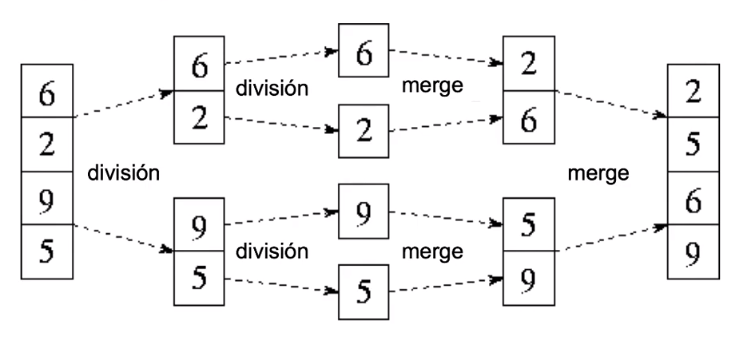
\includegraphics[width=0.7\textwidth]{mergesortEj.png}
    \caption{Ejemplo de MergeSort}
    \label{fig:ejMerge}
\end{figure}

El merge de dos pedazos lo que hace es tener un puntero al primer
elemento de cada pedazo (algoritmo two fingers).
Luego compara cada uno de ellos, lo pone en el arreglo resultado y avanza
dicho puntero (el ganador).
Repite el proceso hasta hacer n-1 pasos, donde n es la cantidad de elementos
entre ambos pedazos.

\paragraph{Complejidades:}
Viendo el merge podemos ver que tiene complejidad O(n-1).
Por otra parte el MergeSort tiene complejidad T(n), y cada parte recursiva
es 2T(n/2).
Si desarrollamos T(n) recursivamente podemos llegar a que no pueda
hacer mas divisiones.
Esto va quedando siempre con terminos de $2^iT(\frac{n}{2^i})+in-2^{i-1}-...-2-1$.
Esto termina con i=log(n) ya que es cuando se cumple que $2^i=n$.
Y esto es O(nlog(n)).

Es estable.
\subsection{Quick Sort}
Es un algoritmo con la metodologia de Divide and Conquer.
Es similar a Merge Sort, pero usando un elemento de pivote.
Es decir separo en dos pedazos, en donde uno tiene los elementos mas chicos
que el pivote y otro que tiene los elemenos mas grande.
Uso esto de forma recursiva hasta no poder dividir mas.
Al hacer esto queda ordenado.

Idealmente quiero siempre elegir como pivote el mediano.
Pero eso en la practica hace que la busqueda del mismo genere
que el algoritmo sea O(nlog(n)) pero con una constnate muy grande.

\begin{figure}[h!]
    \centering
    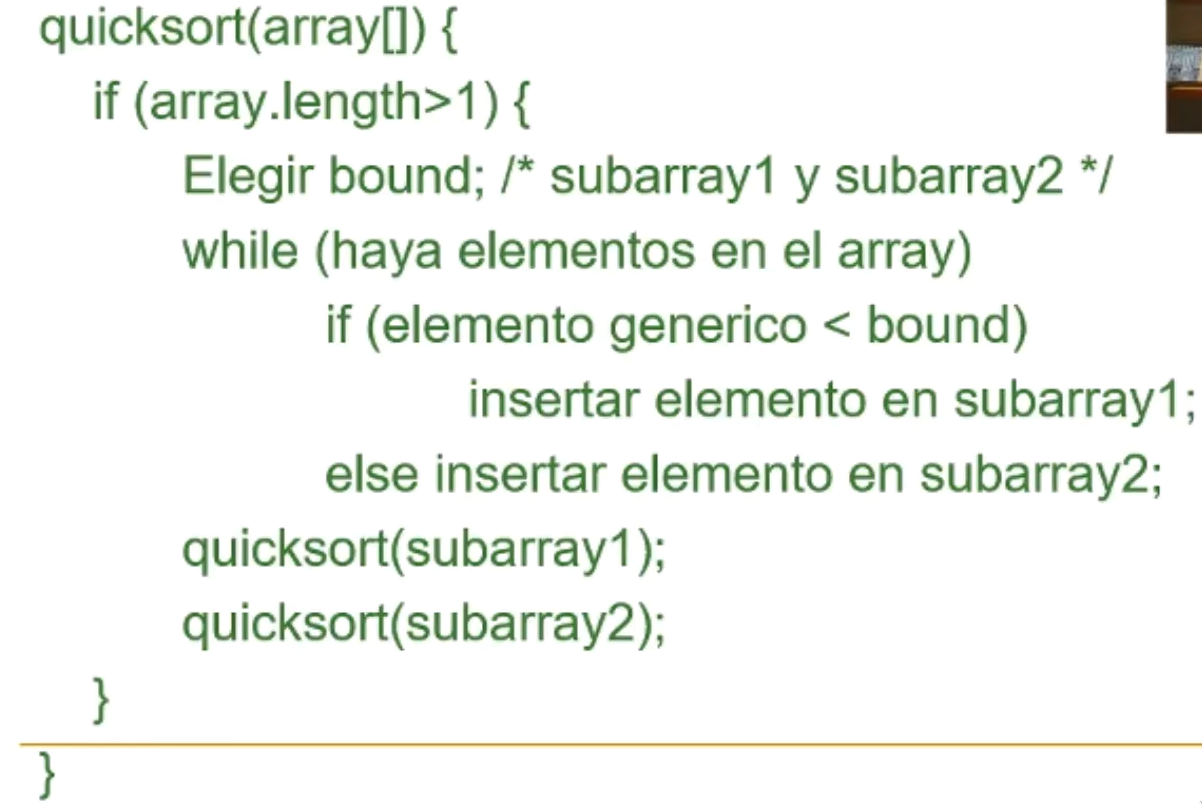
\includegraphics[width=0.7\textwidth]{quicksort.png}
    \caption{Pseudo-codigo del algoritmo de quick sort}
    \label{fig:quicksort}
\end{figure}

\paragraph{Eficiencia:}
Para que sea eficiente se requieren varios trucos.
Por un lado se busca el maximo de todo el arreglo y se lo ubica
al final del arreglo (solo en la primer iteracion).
Esto sirve para que \textit{lower} (ahora lo definimos) no se pueda ir fuera de rango.
La eleccion del pivote se elije simplemente con el elemento central
(el que esta en el medio del arreglo).
El pivote swapea con el primer elemento.
Por otro lado vamos a tener dos iteradores que recorrer de forma ''simultanea''.
Uno compara de izquierda a derecha, \textit{lower} que arranca
en el pirmer elemento que no es el pivote y el otro de derecha a izquierda,
\textit{upper} quye arranca en el ultimo elemento que no es el maximo (anteultimo).
\textit{lower} va ir preguntando si el elemento donde esta es menor que
el pivote y en caso de serlo avanza.
Si se encuentra con un elemento que es mayor frena y se queda ahi.
Con \textit{upper} hace lo mismo pero preguntando si el elemento es mayor.
Cuando ambos estan frenados, swapea ambos elementos y ahi continuan
moviendose desde donde habian frenado.
Cuando \textit{lower} y  \textit{upper} se cruzan se acaba la iteracion.
Swapeo el pivote con el ultimo elemento aputado.


\paragraph{Complejidades:}
En el peor caso es O($n^2$). Pero en caso promedio y mejor caso
es costo O(nlog(n)).

Para esto la eleccion del pivote es al azar.
Algunas implementaciones toman algunos elementos finitos del arreglo
(ej: uno al principio otro en el medio y otro al final) y se toma
al mediano de estos.

No es estable.

\subsection{Counting Sort}
Basicamente me creo un array de tama\~no igual al maximo elemento de mi
arreglo (en general funciona para numeros enteros).
Obviamente requiero tener una cota superior de mis elementos.
Voy mirando mi arreglo y sumo uno a la posicion del elemento que estoy viendo.
Lo itero hasta finalizar mi arreglo.
Podria tambien hacerlo en un dado rango que tiene como menor elemento d y
mayor elemento k.
Entonces tener un array de k-d elementos.

\begin{figure}[h!]
    \centering
    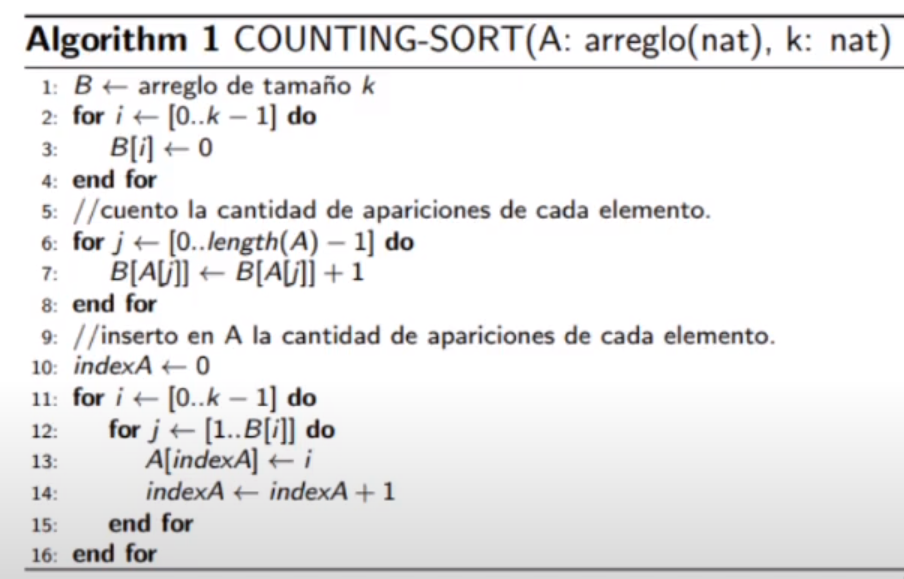
\includegraphics[width=0.7\textwidth]{countingSort.png}
    \caption{Pseudo-codigo del algoritmo de Counting Sort}
    \label{fig:counting}
\end{figure}

Al tener ahora un arreglo de muchas posiciones donde tiene el
numero de apareciciones, basicamente esto ya tiene un orden.
Recorro este vector y voy agregando de forma ordenada los elementos que
tienen apariciones.
Si esta repetido lo agrego esa cantidad de veces.

\paragraph{Complejidades:}
Basciamente es O(n+k).
Donde n es el tama\~no original de mi arreglo, y k es el
tama\~no del otro (k'-d en caso de que tenga un rango).

\subsection{Bucket Sort}
Supone que los elementos pueden separarse en categorias ordenadas.
Se arma M listas y agrega a los elementos segun el criterio.
Luego se hace algun sort (no especifica cual) en cada lista.
Finaliza concatenando todas.

La gracia de bucket sort se da cuando la distribucion de los elementos
de la lista que queremos ordenar es uniforme con respecto a las categorias.
Ejemplo:
Quiero hacer 4 buckets, de 0 a 10, de 10 a 100 , de 100 a 1000 y mas de 1000.
Lo que quiere decir es que hay la misma cantidad de elementos entre
0 a 10, que entre 10 a 100,  que entre 100 a 1000 y mayores a 1000.

\begin{figure}[h!]
    \centering
    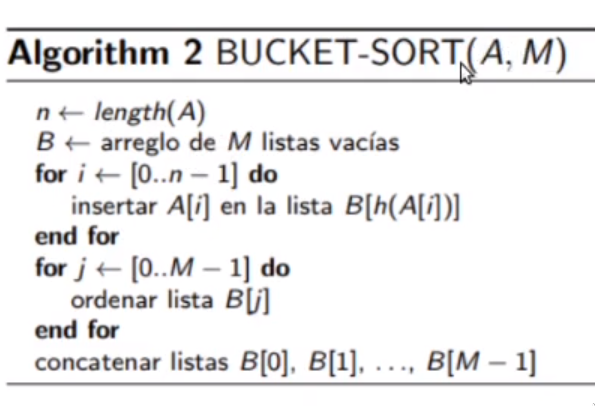
\includegraphics[width=0.7\textwidth]{bucketSort.png}
    \caption{Pseudo-codigo del algoritmo de Bucket Sort}
    \label{fig:bucket}
\end{figure}


\end{document}
